% Алгоритм обратного проецирования (BP).

Рассмотрим задачу восстановления исходной функции по ее Радон-образу. Если рассматривать модель непрерывного мира, то $f(x, y)$ может быть восстановлена при помощи \textbf{обратного проецирования} (\textbf{Back-projection}):
\begin{equation}
\label{backprojection}
    \left[ \mathcal{B}(p_\theta(s)) \right](x, y) = \int_0^{\pi} p_\theta\left( x\cos\theta + y\sin\theta \right) d\theta.
\end{equation}

\begin{figure}[!h]
    \centering
    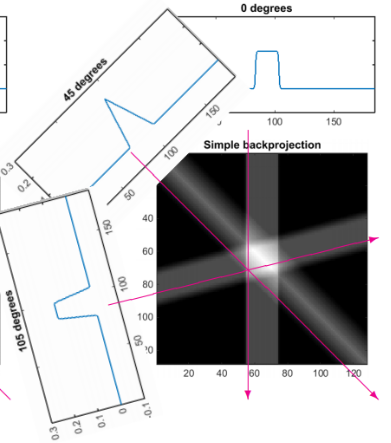
\includegraphics[width=0.5\linewidth]{backprojection_concept}
    \caption{Суть backprojection в одной картинке}
\end{figure}

Выражение \eqref{backprojection} не совпадает с $f(x, y)$, однако часто используется как его приближение.
% source of proof: https://www.desy.de/~garutti/LECTURES/BioMedical/Lecture7_ImageReconstruction.pdf
\begin{gather*}
    f(x, y) =
    \mathcal{F}_2^{-1} \left[ F(u, v) \right](x, y) =
    \int_{\mathbb{R}^2} F(u, v) e^{2\pi i (xu + yv)} du dv = \dots
\end{gather*}

Перейдем в последнем равенстве к полярным координатам по переменным интегрирования: $u = \omega\cos\theta, v = \omega\sin\theta, du dv = |\omega| d\omega d\theta$:
\begin{gather*}
    \dots =
    \int_{0}^{\pi} \int_{-\infty}^{\infty} F(\omega\cos\theta, \omega\sin\theta) e^{2\pi i \left( x \cos\theta + y\sin\theta \right)\omega} |\omega| d\omega d \theta = \dots
\end{gather*}

Используем теорему \ref{fourier_slice_thm} для замены $F(\omega\cos\theta, \omega\sin\theta) = \hat{p}_{\theta}(\omega)$. Также введем для краткости обозначение $s = x\cos\theta + y\sin\theta$.
\begin{gather*}
    \int_{0}^{\pi} \int_{\mathbb{R}} |\omega| \hat{p}_{\theta}(\omega) e^{2\pi i s \omega} d\omega d\theta =
    \int_{0}^{\pi} \left[ \mathcal{F}^{-1} \left( |\omega| \hat{p}_\theta(\omega) \right) \right](s) d\theta.
\end{gather*}

Если удалить из последнего выражения якобиан $|\omega|$, оставив под интегралом вместо выражения $\mathcal{F}^{-1}\left[ \hat{p}_\theta(\omega) \right](s) = p_\theta(s) = p_\theta\left( x\cos\theta + y\sin\theta \right)$ то получится в точности выражение \eqref{backprojection}.
